%!TEX TS-program = lualatex
%!TEX encoding = UTF-8 Unicode
%% (this document must be compiled with LuaLaTeX) 
%% Main file for PFPE gravimeter documentation
%% 
%% Formatting loosely based on the Overleaf Software Manual and Technical Document Template	
%% 									

\documentclass{pfpe-manual}

% Packages used in this example
\usepackage{graphicx}  % for including images
\usepackage{microtype} % for typographical enhancements
\usepackage[letterpaper,top=4.2cm,bottom=4.2cm,left=3.5cm,right=3.5cm]{geometry} % for setting page size and margins

% Custom macros used in this example document
\newcommand{\doclink}[2]{\href{#1}{#2}\footnote{\url{#1}}}
%\newcommand{\cs}[1]{\texttt{\textbackslash #1}}

% Frontmatter data; appears on title page
\title{gravitron manual}
\version{1.0.0}
\author{Hannah F. Mark}
\license{CC-BY 4.0}
%%%%%%%%%%%%%%%%%\softwarelogo{\includegraphics[width=8cm]{figs/grav_photo}}

\begin{document}

\maketitle

\tableofcontents
\newpage

\section{Introduction}

gravitron is a GUI software tool for recording gravity ties and calculating meter biases. It is designed for the Potential Fields Pool Equipment (PFPE) DGS gravimeters used onboard UNOLS vessels.

\section{Installation}
\label{install}
gravitron is an electron app for node.js v20+. If you read that last sentence and thought ``ok, I know what to do with that'' then feel free to grab the source code (\url{https://github.com/PFPE/gravitron}), and build/run it as you would any similar program on your operating system of choice. If you're not as used to programs like this, read on for some instructions.

\subsection{Option 1: Packaged app}
There are packaged applications for linux, Mac OS, and Windows available on the github releases page (\url{https://github.com/PFPE/gravitron/releases}). These will likely work well on linux, but may or may not properly install on Mac OS or Windows because they are not ``official'' applications distributed through Apple or Microsoft app stores. We promise there's nothing malicious in there, so if you can convince your computer to install from one of these packages, that's the simplest option. You can then run gravitron as you would any other application. If that doesn't work for you, go to Section \ref{runwithnode} for an alternative.

\subsubsection{Linux app}
The github releases page has .rpm and .deb packages. For Ubuntu, download the .deb package and install either with software installer or by running \texttt{sudo dpkg -i /path/to/deb/file}.

\subsubsection{Windows app}
The packaged .exe installer has been tested on Windows 11 and it seems to work! When you download and run the installer you will likely see a system prompt warning you that the program does not have a verified author. If you click on the ``more info'' button it should let you tell it to install anyway. Once it has installed and opened the application, pinning the app to the taskbar is recommended to make it easier to find later. Otherwise, the executable can be found at: 

\texttt{C\textbackslash :Users\textbackslash (yourname)\textbackslash AppData\textbackslash Local\textbackslash gravitron\textbackslash app-1.0.0\textbackslash gravitron.exe}. 

\noindent \texttt{AppData} is a hidden folder.

\subsubsection{Mac app}
Download the darwin arm64 zip file from the releases page, and good luck.

\subsection{Option 2: Run the code on your own}
\label{runwithnode}
The gravitron source code contains all the necessary pieces and instructions to install dependencies and run locally, provided you have node.js on your system. So, here's how you do it:
\begin{itemize}
    \item Install node and npm on your computer (instructions at \url{https://nodejs.org/en/download}). In a terminal (or powershell), make sure that if you run \texttt{node -v} and \texttt{npm -v}, the commands return version numbers for node and npm.
    \item Download the gravitron source code from \url{https://github.com/PFPE/gravitron} and unpack the files somewhere.
    \item Navigate to those files in a terminal/powershell.
    \item In that directory (contains package.json and other files), run the command \texttt{npm ci}. This will install the dependencies for gravitron.
    \item In the same directory, run the command \texttt{npm start} to run the gravitron application. 
\end{itemize}


\section{Using gravitron}

\begin{figure}[ht!]
\centering
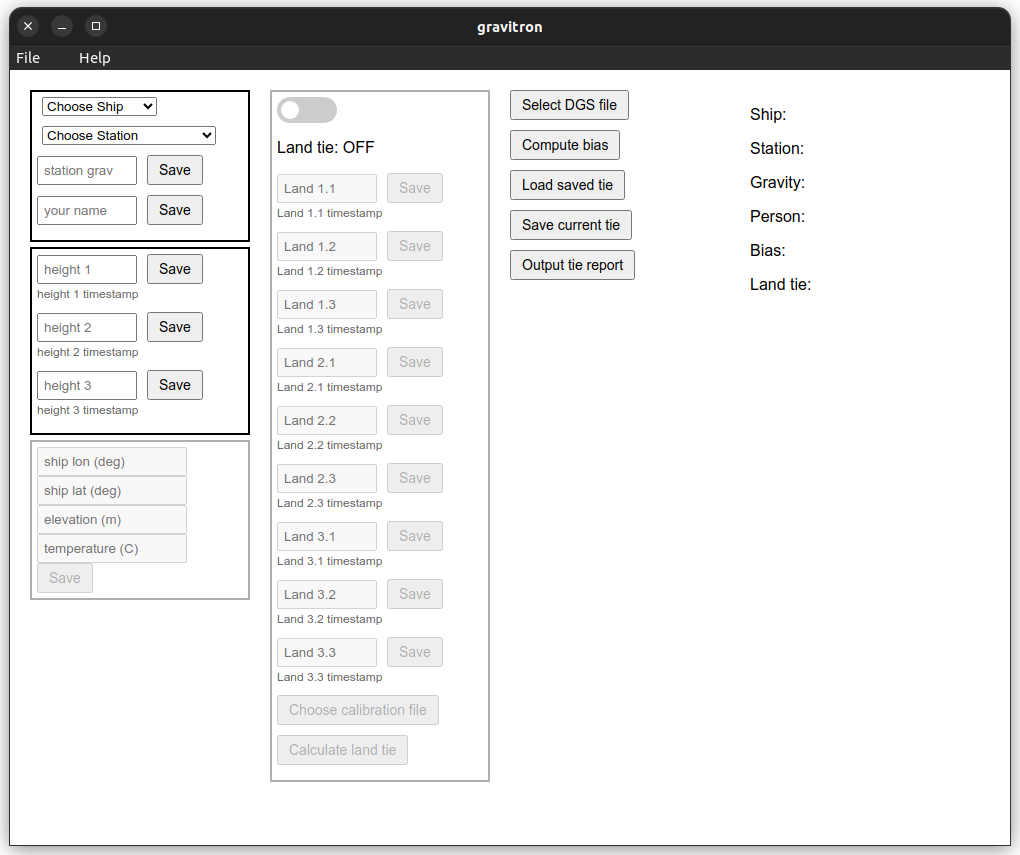
\includegraphics[width=\textwidth]{figs/gravitron_window.png}
\caption{The gravitron window.}
\label{fig:window}
\end{figure}

\subsection{Intro to the gravitron window}

The gravitron window (Figure~\ref{fig:window}) has 4 columns. The columns contain, from left (col 1) to right (col 4):
\begin{enumerate}
\item Ship/station metadata entry, water height entry, land tie metadata entry
\item Land tie count measurement entry, meter calibration file selection
\item Buttons for choosing DGS data files, computing bias, saving/loading tie files, and writing out tie reports
\item Status messages
\end{enumerate}

\noindent
Buttons and fields for land tie information and actions will appear greyed out unless the land tie toggle button is set to "on".

\subsection{Steps for taking a tie}
\label{tie-instructions}
\begin{enumerate}
\item Start the gravitron program (see Section~\ref{install})
\item Enter the tie metadata
    \begin{itemize}
    \item Select a ship from the dropdown menu.
    \item Select a station from the dropdown menu. This will populate the input field below the menu with the gravity value for that station. If you choose `Other', you will need to change the value in that input field and press save. The station gravity value to be used for the tie will appear in the status column on the right side of the window.
    \item Enter the name of the tie-taker in the input field labeled `your name' and save it.
    \end{itemize}
\item \textbf{For land ties only:} Click the land tie toggle switch to the `on' position, and enter land meter metadata
    \begin{itemize}
    \item Enter the coordinates of the ship (where you will be taking the land tie) in decimal degrees, the elevation in meters, and the temperature in degrees C, and press `save'. Note that you can leave fields blank and fill in the information later in the report or the saved tie.
    %\item Select a land meter from the dropdown and press `Save'. 
    %\item If you choose `Other', you will need to enter the meter name and will also need to supply a calibration file for the meter. Use the `Other cal. file' button to select the calibration file (see Section~\ref{datab}).
    \end{itemize}
\item Make pier water height measurements
    \begin{itemize}
    \item Measure water height at the pier 3 times, with \textasciitilde 30 minutes elapsing between measurements. Enter each water height (in meters) in the appropriate field in gravitron, and press the corresponding `save' button. The timestamp for each measurement will appear below the field where the water height is entered.
    \item[\textbf{Note:}] Pressing `save' tells gravitron that the measurement was taken at the \textit{current time} when the button is pressed. If you aren't saving the water height measurements at the time they are taken, see Section ~\ref{later} for instructions on adjusting timestamps.
    \end{itemize}
\item \textbf{For land ties only:} Measure counts with the land meter
    \begin{itemize}
    \item Measure counts on the ship three times, recording and saving measurements in gravitron
    \item Measure counts at the station three times, recording and saving measurements in gravitron
    \item Again, measure counts on the ship three times, recording and saving measurements in gravitron
    \item[\textbf{Note:}] Pressing `save' tells gravitron that the measurement was taken at the \textit{current time} when the button is pressed. If you aren't saving the counts measurements at the time they are taken, see Section ~\ref{later} for instructions on adjusting timestamps.
    \end{itemize}
\item Use the `Select DGS file' button to select the file containing `laptop' data for the time period when the water height measurements were taken. You can select multiple files.
\item \textbf{For land ties only:} Use the `Choose calibration file' button to load a meter calibration file. Then, use the `compute land tie' button to compute the land tie value
\item Use the `Compute bias' button to do the bias calculation.
\item Use the `Output tie report' button to save the gravity tie report
\item \textbf{Optional, recommended:} Use the `Save current tie' button to save the tie to a toml file. This is a file that gravitron can re-read later if any parameters need to be adjusted.
\end{enumerate}

\subsubsection{What if I made my tie measurements before running gravitron?}
\label{later}
This is fine, as long as you recorded the (UTC) times at which those measurements were taken.

Follow the steps in Section~\ref{tie-instructions} up to step 4 (or step 5 if taking a land tie). Then, use the `Save current tie' button to save the info to a file (NOT a report; see Section~\ref{save-re}). 

Open the file you just saved (with the extension .toml) in a text editor (NOT word; notepad or textedit or gedit should be ok). Edit the timestamps for each of your measurements (water heights and/or land meter counts) to match when the measurements were actually taken. Make sure that the times you put in the file are in UTC and that they match the timestamp formatting in the original toml file. Save the toml file. 

Then, back in gravitron, use the `Load saved tie' button to read the edited toml file. This will load all of your measurements with the correct timestamps. Resume the Section~\ref{tie-instructions} sequence at step 6.

\subsubsection{When do I need to do a land tie?}
Land ties are only necessary when the nearest station with a known gravity measurement is not right next to where the ship is docked -- specifically, if the station is more than 50m away from the ship. Gravity is measured with a calibrated meter on the ship, at the station, and then on the ship again, and those measurements are used to calculate an absolute gravity measurement for the ship's location that is referenced to the established station value.

\subsection{Saving and re-reading ties}
\label{save-re}
gravitron has two buttons, `Save current tie' and `Load saved tie', that enable writing and reading tie information to simple text files separate from tie reports. These files, with the extension .toml, contain key=value pairs for tie information. Things that have not (yet) been entered or calculated in gravitron when a toml file is written will have placeholder values.

You can use this save/load capability to pause and resume working on gravity ties without having to keep the gravitron program open (see also:~\ref{later}). You can also use saved toml files to check that the values gravitron is using for calculations are consistent and correct. 

Note that gravitron doesn't automatically save or read toml files -- it only touches those files when you press the save/load buttons. Any changes made after loading a saved tie are not reflected in the toml file unless you save the tie again.

\subsection{Database files}
\label{datab}
gravitron ships with a set of text files with that contain some information on UNOLS ships, stations with known gravity measurements, and calibration tables for some land meters. Some of these files are automatically read by the program; the meter calibration files may be loaded by the user when a land tie is done.

The ship is used in gravitron to determine how DGS files are read. While most UNOLS ships with DGS gravimeters write out `laptop' data files in a common format, there are some exceptions, and we've done our best to accommodate file format differences but we can't plan for ships that we don't know about. So, if you select a ship that we don't yet know the file format for, you will not be able to read in a DGS file. You can still record tie measurements and write them out in a toml file, and bias can be calculated later once you or we have figured out how to read the relevant meter file.

The station where a tie is taken should have an associated absolute gravity measurement, which is what the bias calculation is referenced to. If you choose `Other' for your station, or choose a station which does not have a gravity measurement listed in the database, you will have to enter a number for absolute gravity in gravitron in order to compute bias.

If you are taking a land tie, gravitron will need calibration information for the meter you are using. Calibration files for some meters are included with gravitron and the `Choose calibration file' button should default to the location of those files so you can find them easily. Meter calibration files are plain text files with three columns: count brackets, corresponding mGal values, and offset factors. Values in each row of the file are separated by a space. A calibrated mGal measurement for a count measurement is calculated by finding the closest count bracket less than the measured counts, and then adding together the corresponding mGal value for that bracket and the offset factor for the bracket multipled by the difference between the bracket and the actual counts.

gravitron's files can also be edited/updated with new information. If there are stations, meters, or ships that should be added, please contact PFPE.

\subsection{Debug mode}
\label{nobugs}
The `File' menu has an option to toggle debug mode on and off. By default, debug mode is off when gravitron starts. The status column will say `debug off' when debug mode is off, and you will want to keep it off while you are taking a tie. In fact, you'll probably just want to keep it off all the time -- users can safely ignore this setting.

If you turn debug mode on and try to calculate bias with some timestamped water height measurements and some loaded gravimeter data file, gravitron will internally select timestamps for the water height measurments from the times in the data file and use those times for the calculation. This is useful if you want to try out gravitron using a random old data file and don't feel like manually setting timestamps in a toml file to match the data timespan, because gravitron cannot calculate bias unless a data file is loaded that covers the times of the recorded height measurements. However, the resulting bias calculation will not be meaningful at all. 


\section{Why do we take gravity ties?}
If you're curious as to why you are being asked to spend 90+ minutes making water height measurements and clicking buttons on your computer, here's a quick explanation of what gravity ties are for.

\subsection{Marine gravimetry in a nutshell}
Gravimetry is the measurement of the strength of a gravitational field. Gravity is typically measured in units of acceleration, such as the Gal (short for galileo) which is defined as 1 cm/s$^2$. Measuring the marine gravity field, either at the sea surface or at depth, can give us information about seafloor bathymetry, the structure of the crust, plate tectonics, and more: once gravity data is corrected for known or assumed effects, the remaining anomalies can be interpreted in terms of local variations in mass/density in the Earth.

Measuring gravity on a large moving platform (like a ship) is difficult \emph{because} the platform is large and moving. Accurately measuring small variations in acceleration due to gravity requires that we be able to compensate and correct for all the other factors that are trying to accelerate the sensor in the gravimeter. Since the gravimeter isn't perfect and gets shaken around at sea, we also need to account for drift in the sensor's measurements over time. Gravity ties, where the ship gravimeter's measurement is referenced to a known gravity measurement in port, enable us to track meter drift by comparing ties taken before and after a cruise. 

\subsection{How DGS meters work}
DGS gravimeters contain AT1M sensors. The AT1M sensor is a scalar gravity/specific force sensor mounted in a 2-axis gyro stable platform that keeps the sensitive axis of the gravity meter aligned with the local gravity vector. The magnitude of the local gravity vector is measured and recorded. Basically, a mass is suspended by a stable metal spring with low temperature sensitivity, and small variations in local gravity are measured based on the electrical current of a Lorentz force actuator which, together with a position detector, keeps the sensing spring at a constant length as the suspended mass experiences changes in the gravitational force and moves in response.

\section{Help!}
\label{helphelp}

\subsection{Troubleshooting}

\subsubsection{The packaged app doesn't work}
The packaged apps may not install properly because of security features in some operating systems. You may also be using a version of your operating system that differs significantly from the version that packaged app was compiled for. In either case, the easiest solution is probably just to install node.js and run the app from the source files sans packaging. Instructions for this are in Section~\ref{install}.

\subsubsection{I thought I installed node.js but node -v doesn't work??}
This should not apply to anyone who is using the packaged app. If you decided instead to download and run the code separately, and you used fnm in powershell to install node on Windows, you may need to do one extra thing to tell powershell where to find node. The github page for fnm has some instructions for this (\url{https://github.com/Schniz/fnm#shell-setup}). This may also require configuring powershell to allow startup scripts; google it or email PFPE for help.

If the above information does not help you, try checking stackoverflow. If you still can't get it to work, you can try asking PFPE but we may be just as lost as you are.

\subsubsection{gravitron can't read my DGS data files}
First, make sure that you are using the `laptop' data files rather than the raw files, as those are what gravitron is designed to read. If that still doesn't work, contact PFPE with a sample of the unreadable file. It may be that gravitron doesn't yet know how to read files from your ship, as there are variations in gravimeter file format between vessels/instruments. Note that you can take and save all of the measurements necessary for a gravity tie and wait until later to compute the bias if there are issues with reading gravimeter files.

\subsubsection{The calculated bias number is really weird}
There are several possibilities here, but they all boil down to: there's probably some miscommunication between us and the gravitron program. Maybe the timestamps for measurements are incorrect, or the DGS file is not being read properly, or there is some mixup with measurement units. 

You can check some of these possibilities by using the `save current tie' button to write out the info that gravitron has to a toml file, and looking at that file in a text editor. Check to make sure that the timestamps make sense, and that the \texttt{avg\_dgs\_grav} value looks reasonable. Water height measurements should all be in meters, and timestamps must be UTC rather than local time to match what is recorded in the gravimeter files.

Note also that if you try to calculate bias but the DGS data that is loaded into the program does not cover the timespan of your water height measurements, the \texttt{avg\_dgs\_grav} value will default to -99999 so even if the gravity at the pier is calculated correctly the bias will not be.

\subsubsection{I have some other question that's not answered here}
For specific assistance, contact PFPE at \href{mailto:pfpe-internal@whoi.edu}{pfpe-internal@whoi.edu}.

\subsection{Glossary}
\begin{itemize}
\item \textbf{directory} is another word for `folder' on a computer
\item \textbf{toml} stands for \href{https://toml.io/}{Tom's Obvious Minimal Language}. It's a standard for writing human-readable configuration files similar to INI files.
\item \textbf{gravity} is the force that attracts a body toward any other physical body that has mass.
\end{itemize}

\subsection{Contributing to the code}
Do you have ideas for making gravitron better? Go ahead and \href{https://github.com/PFPE/gravitron/issues}{raise an issue} on the github page or, if you're a savvy javascript programmer, submit a pull request. You can also email PFPE at \href{mailto:pfpe-internal@whoi.edu}{pfpe-internal@whoi.edu}u.

\end{document}
